\section{Dataset and Setup}
\label{sec:data}

\begin{figure}[t]
\centering
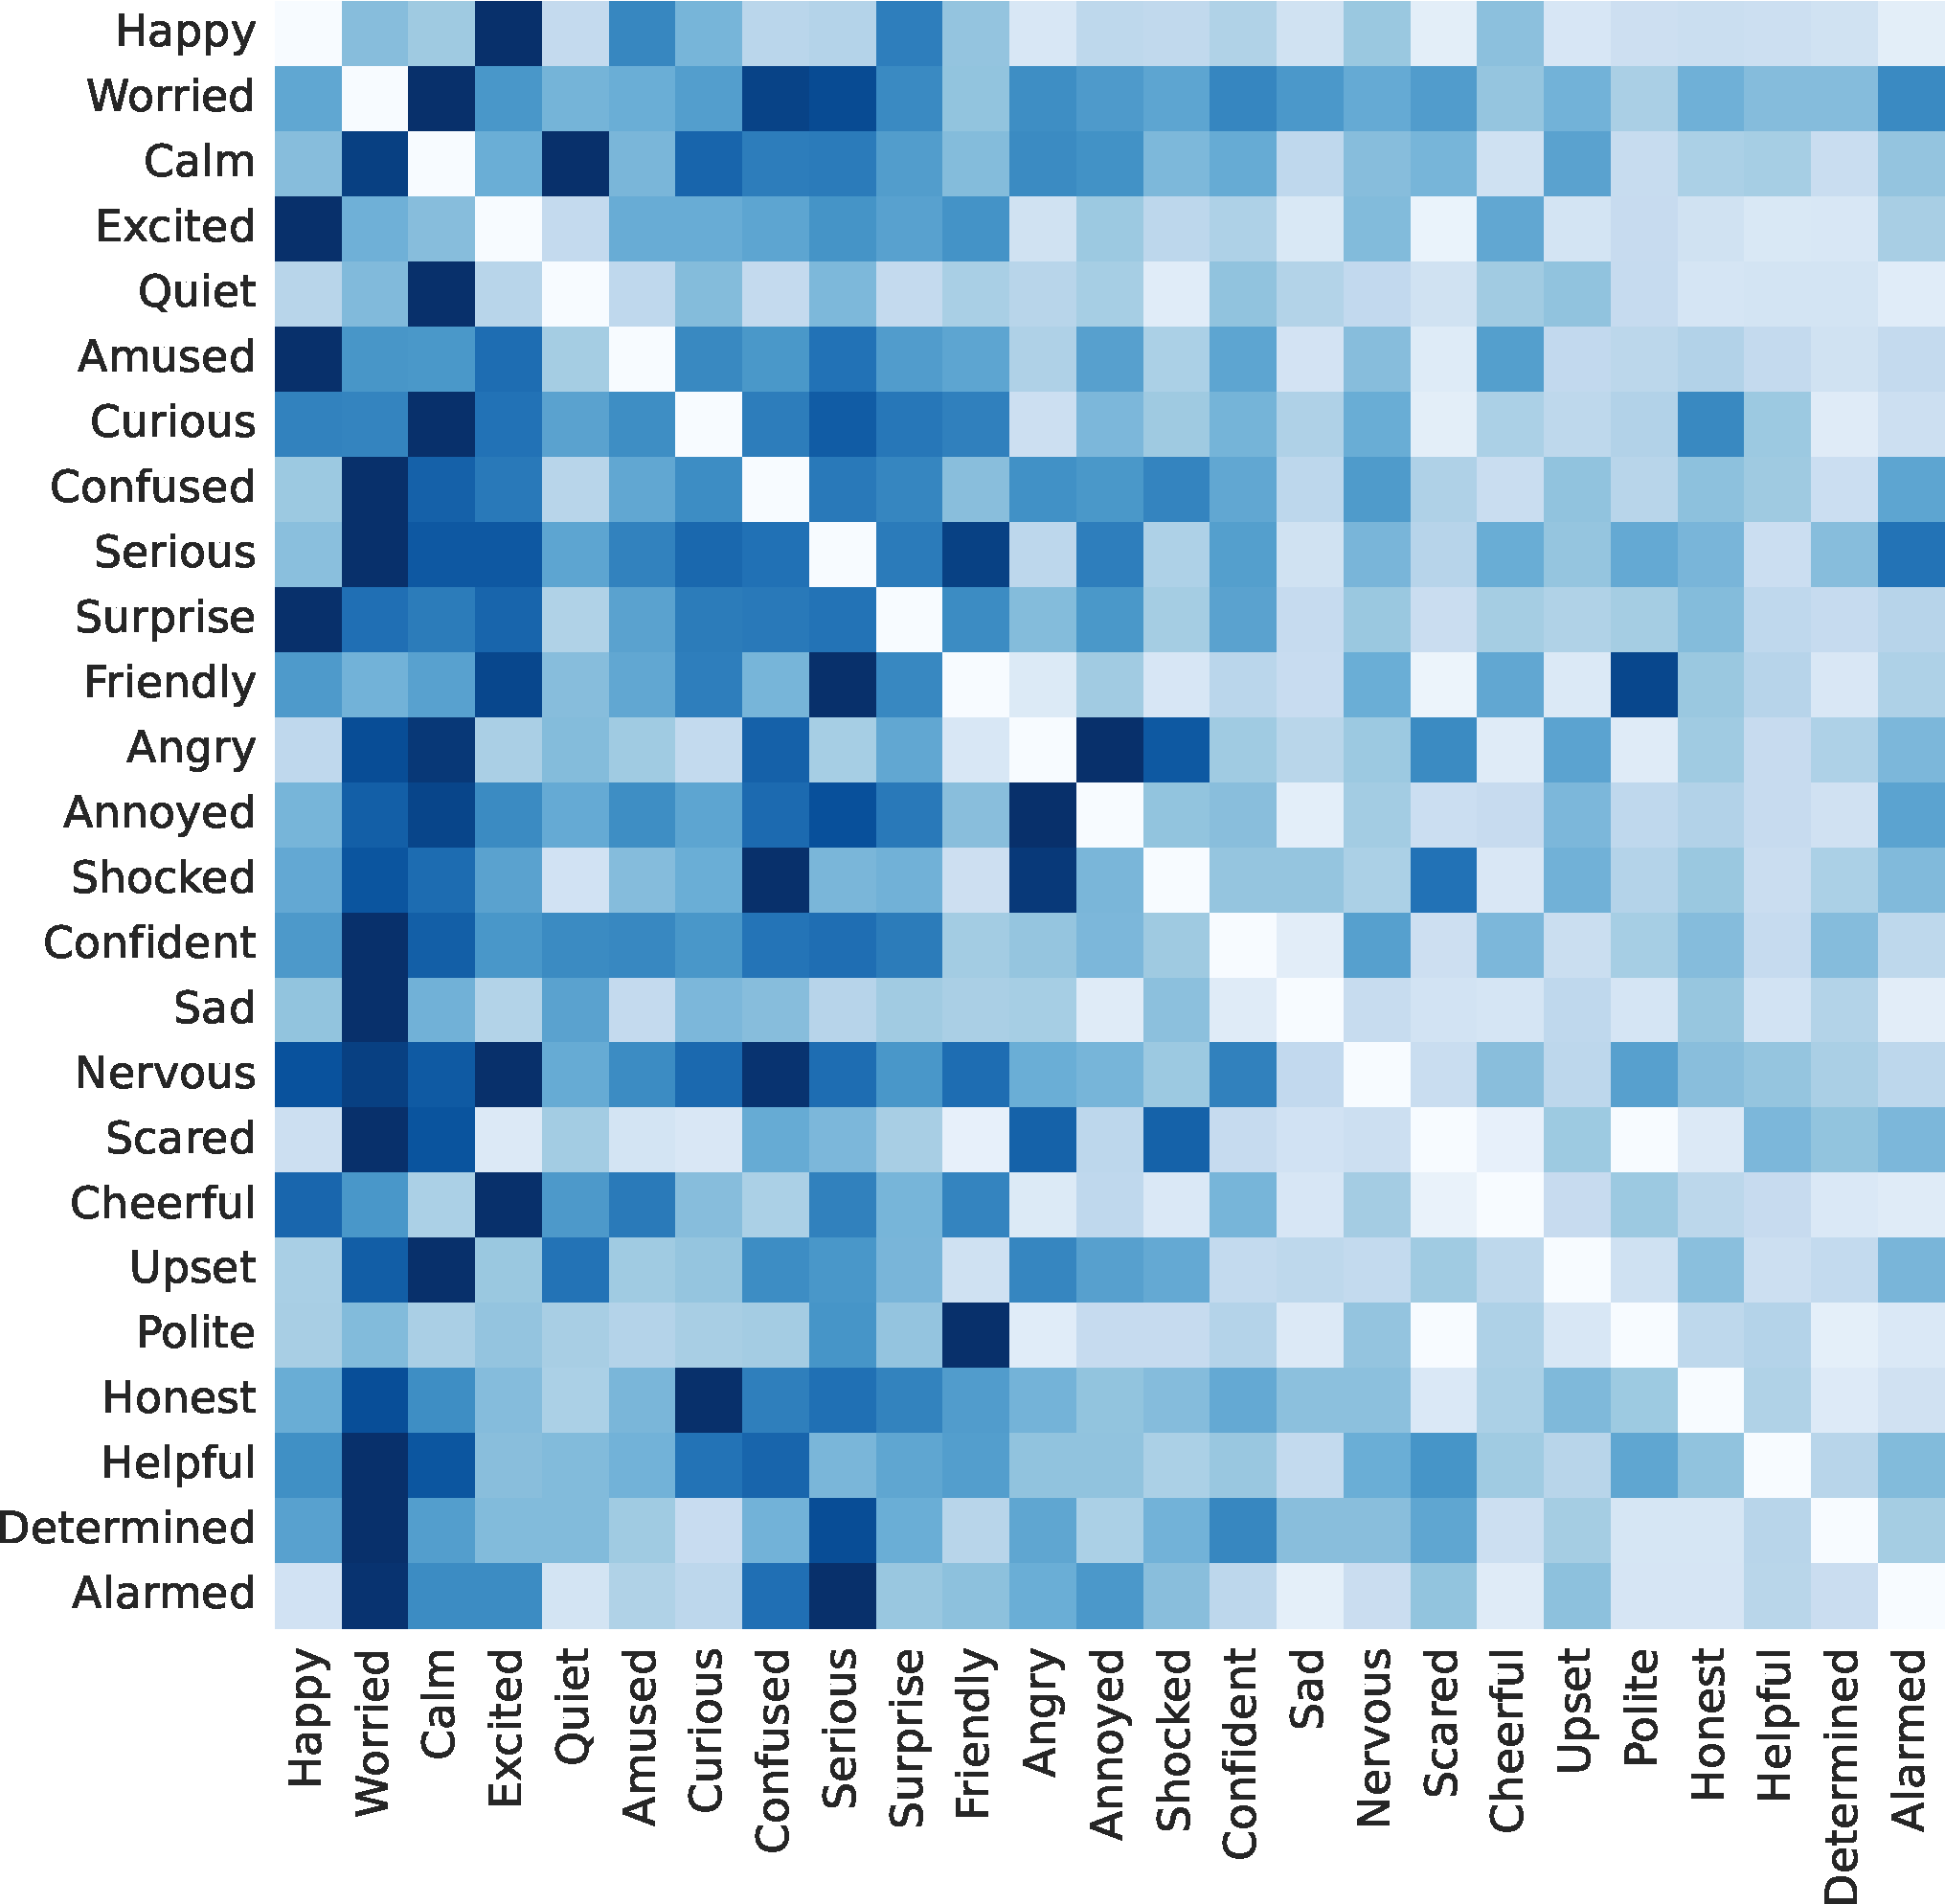
\includegraphics[width=0.48\linewidth]{Figures/scene_25.pdf}
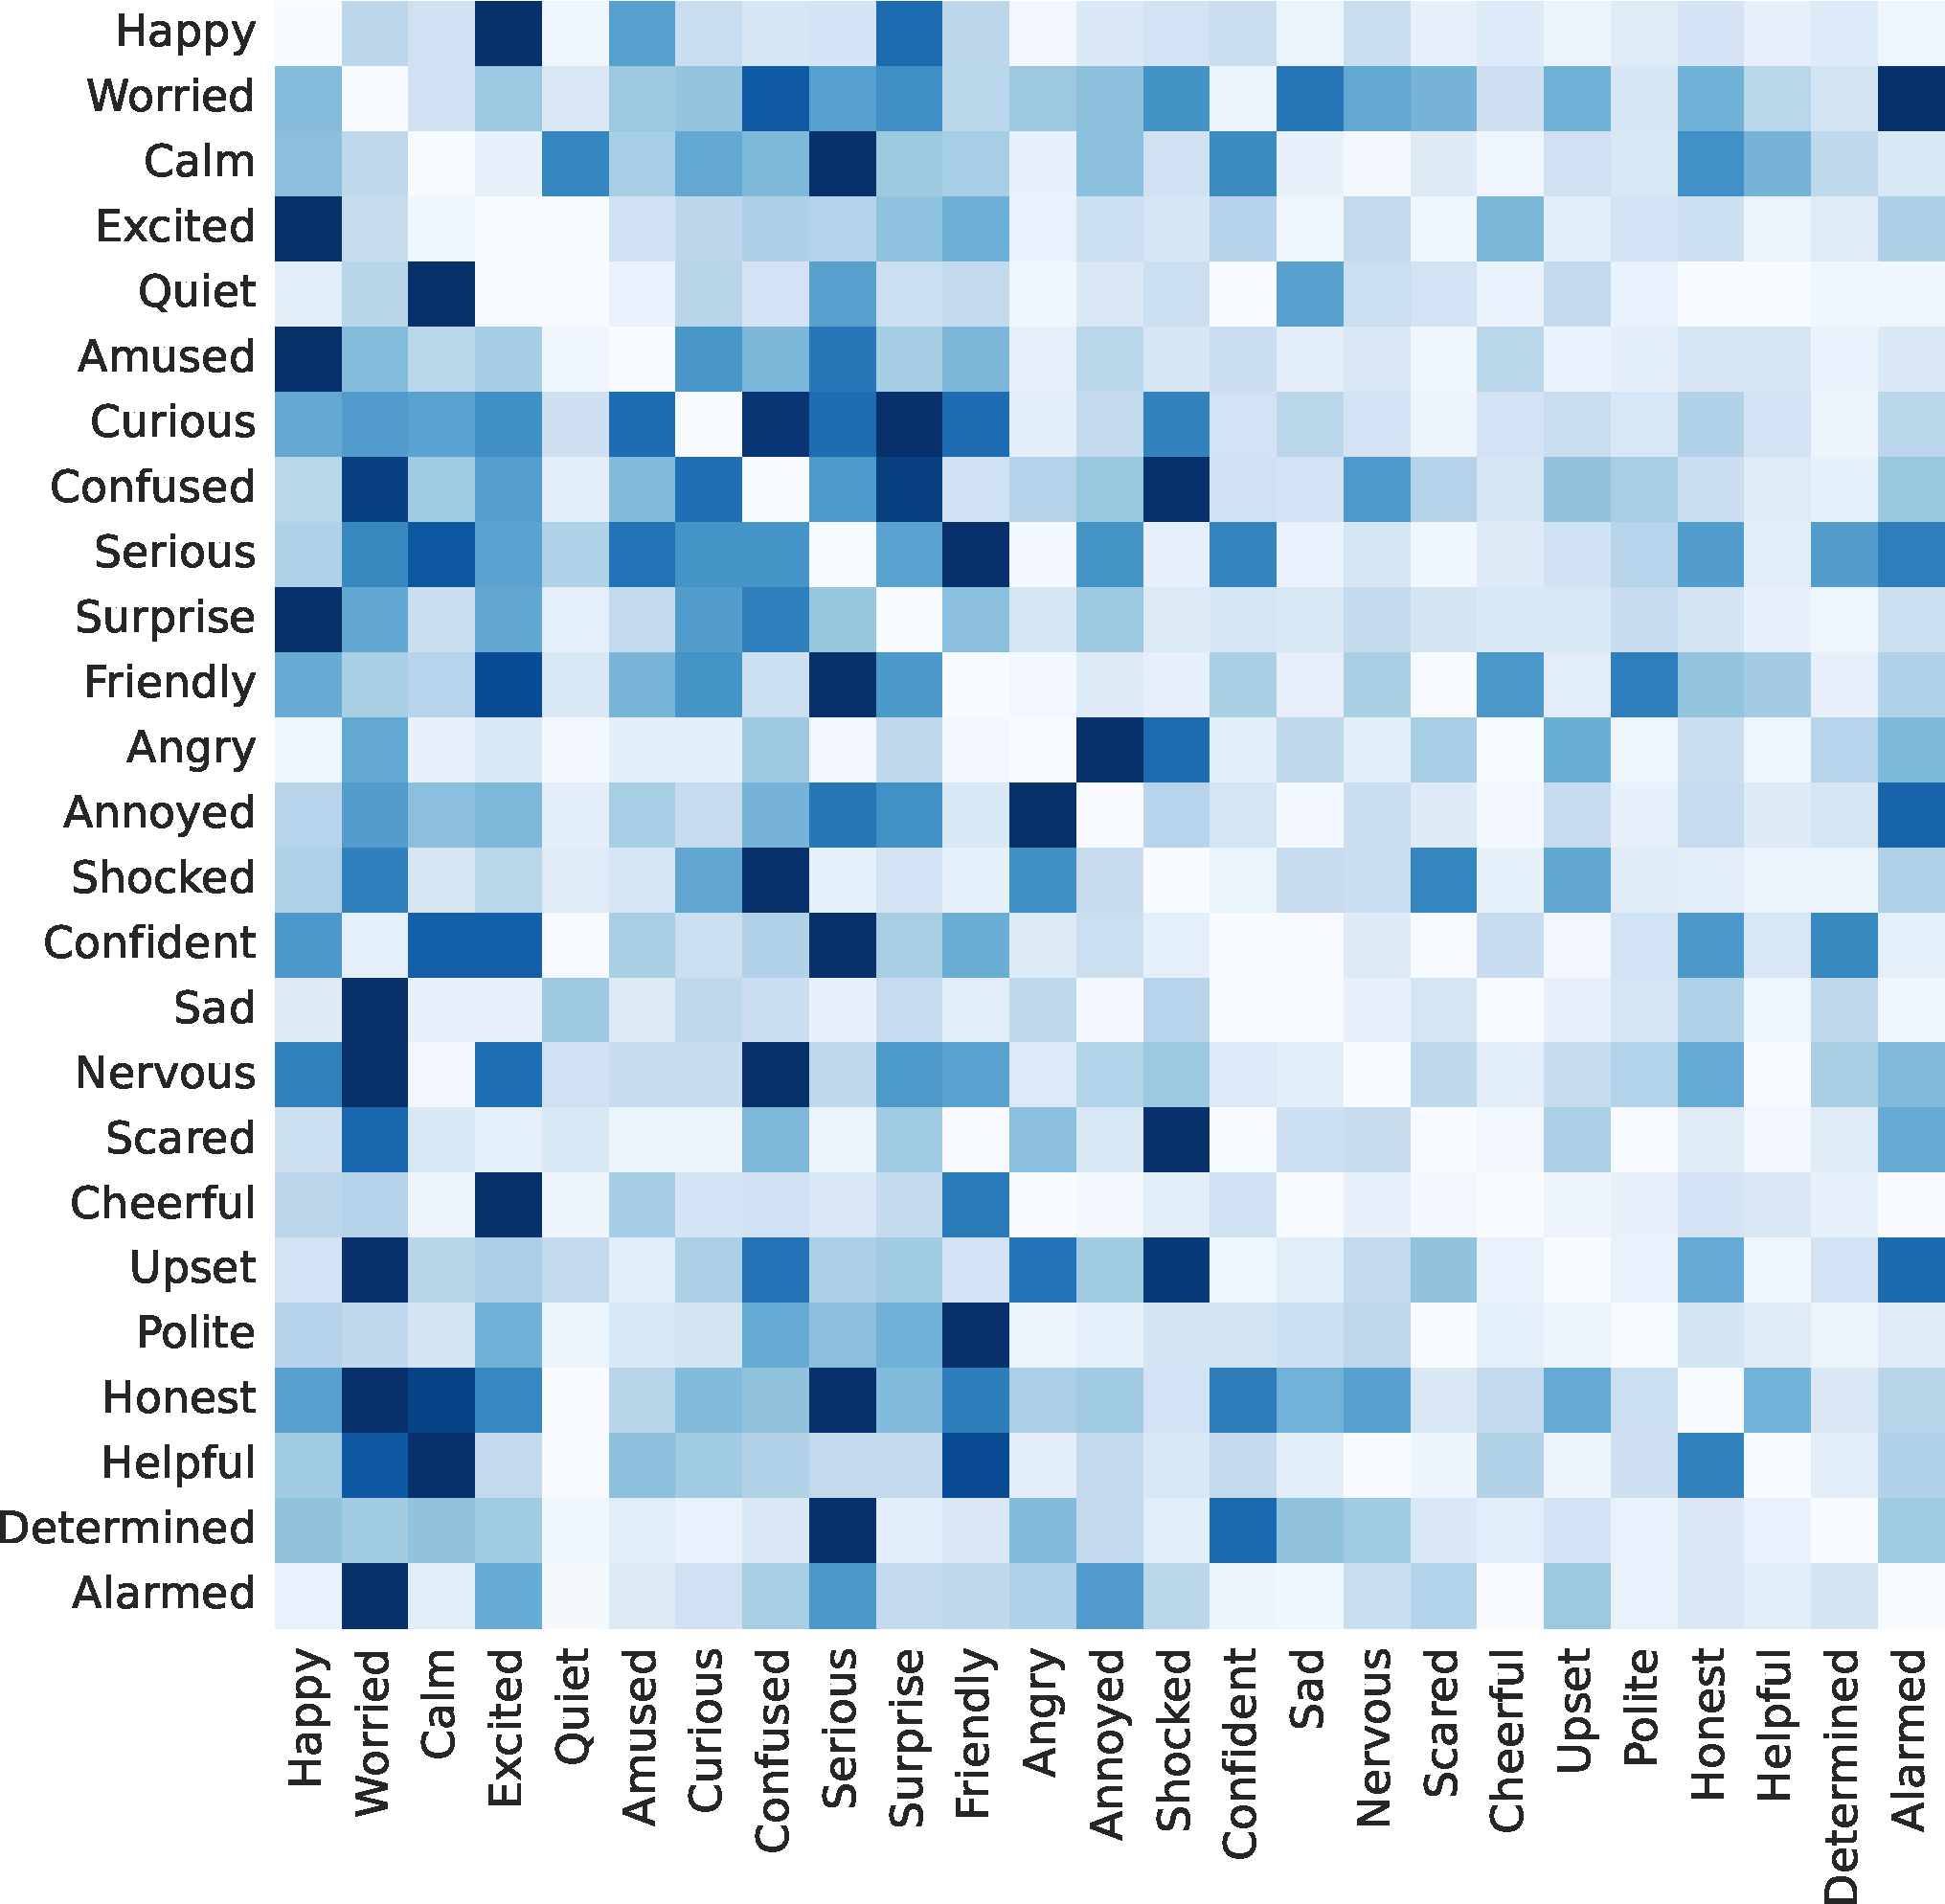
\includegraphics[width=0.48\linewidth]{Figures/characters_25.pdf}
\vspace{-2mm}
\caption{Row normalized label co-occurrence matrices for the top-25 emotions in a \emph{movie scene} (left) or for a \emph{character} (right).}
\vspace{-4mm}
\label{fig:cooccurrence_maps}
\end{figure}

\begin{figure}[t]
\centering
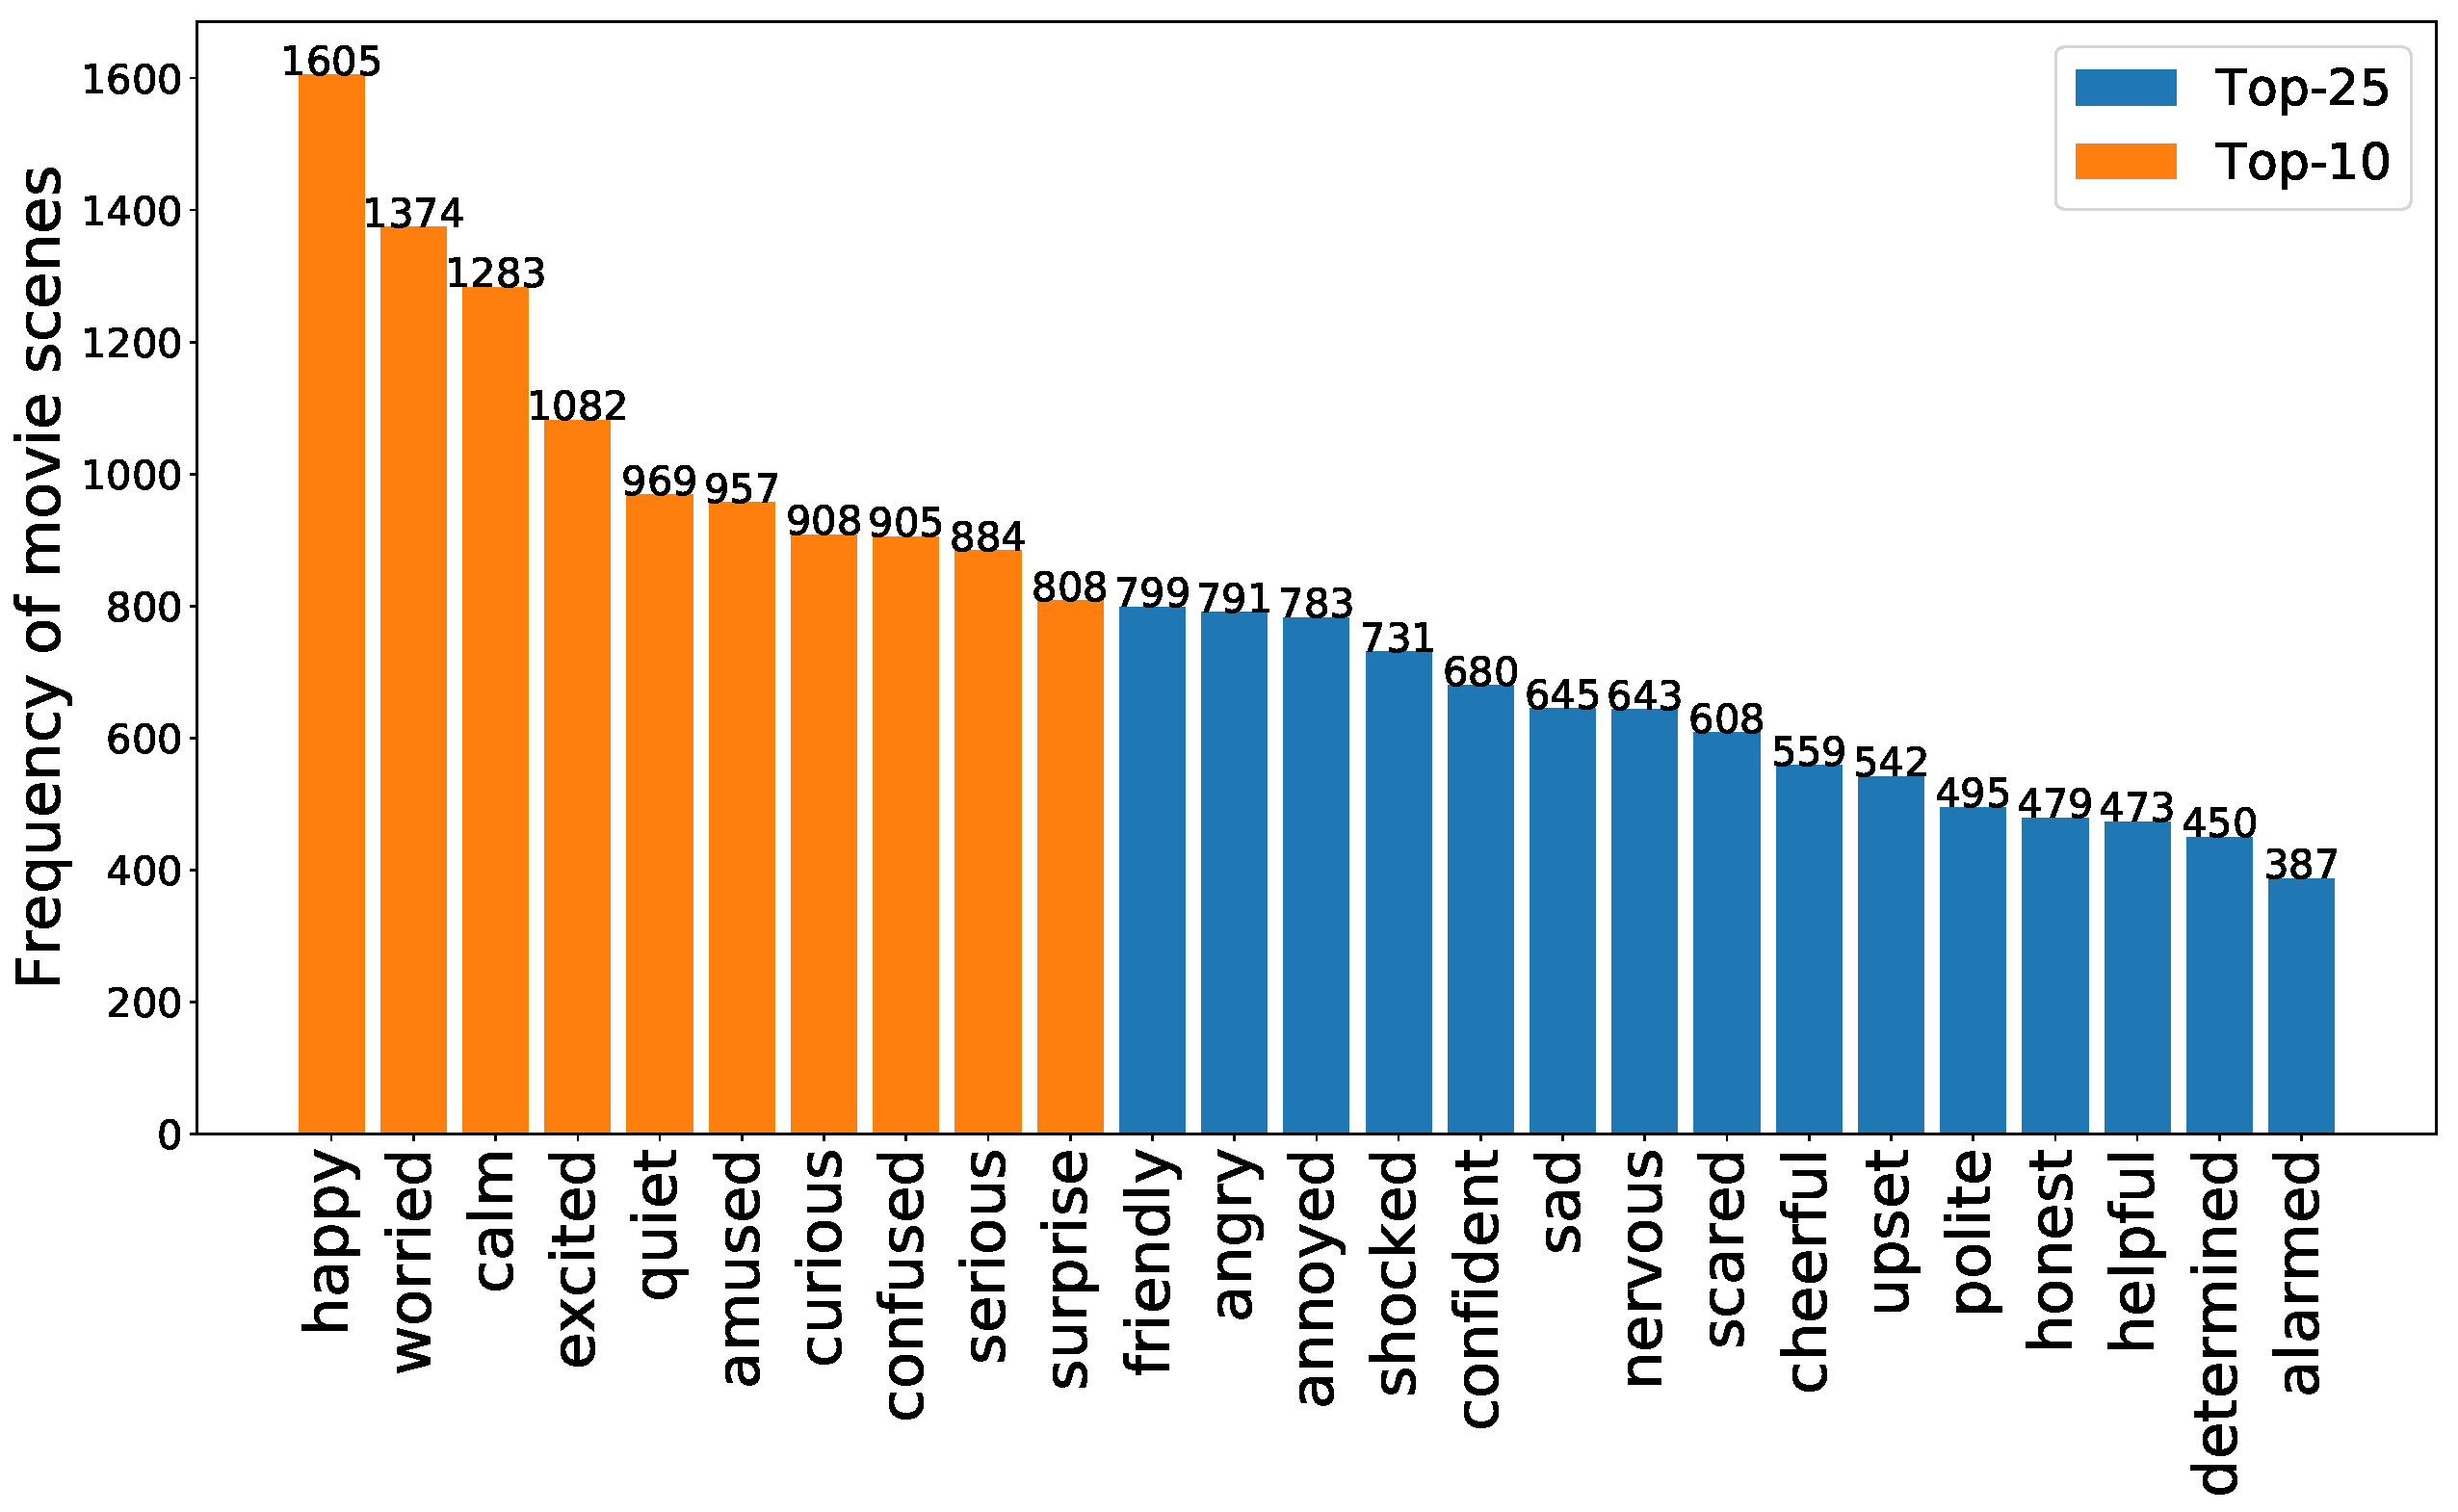
\includegraphics[width=0.6\linewidth]{Figures/top_10_25_emo_freq.pdf}
\vspace{-2mm}
\caption{Number of movie scenes containing top-10 and 25 emotions. Note, the top-25 label set includes the top-10 emotions.}
\vspace{-5mm}
\label{fig:emotionFrequency}
\end{figure}

\begin{figure}[t]
\centering
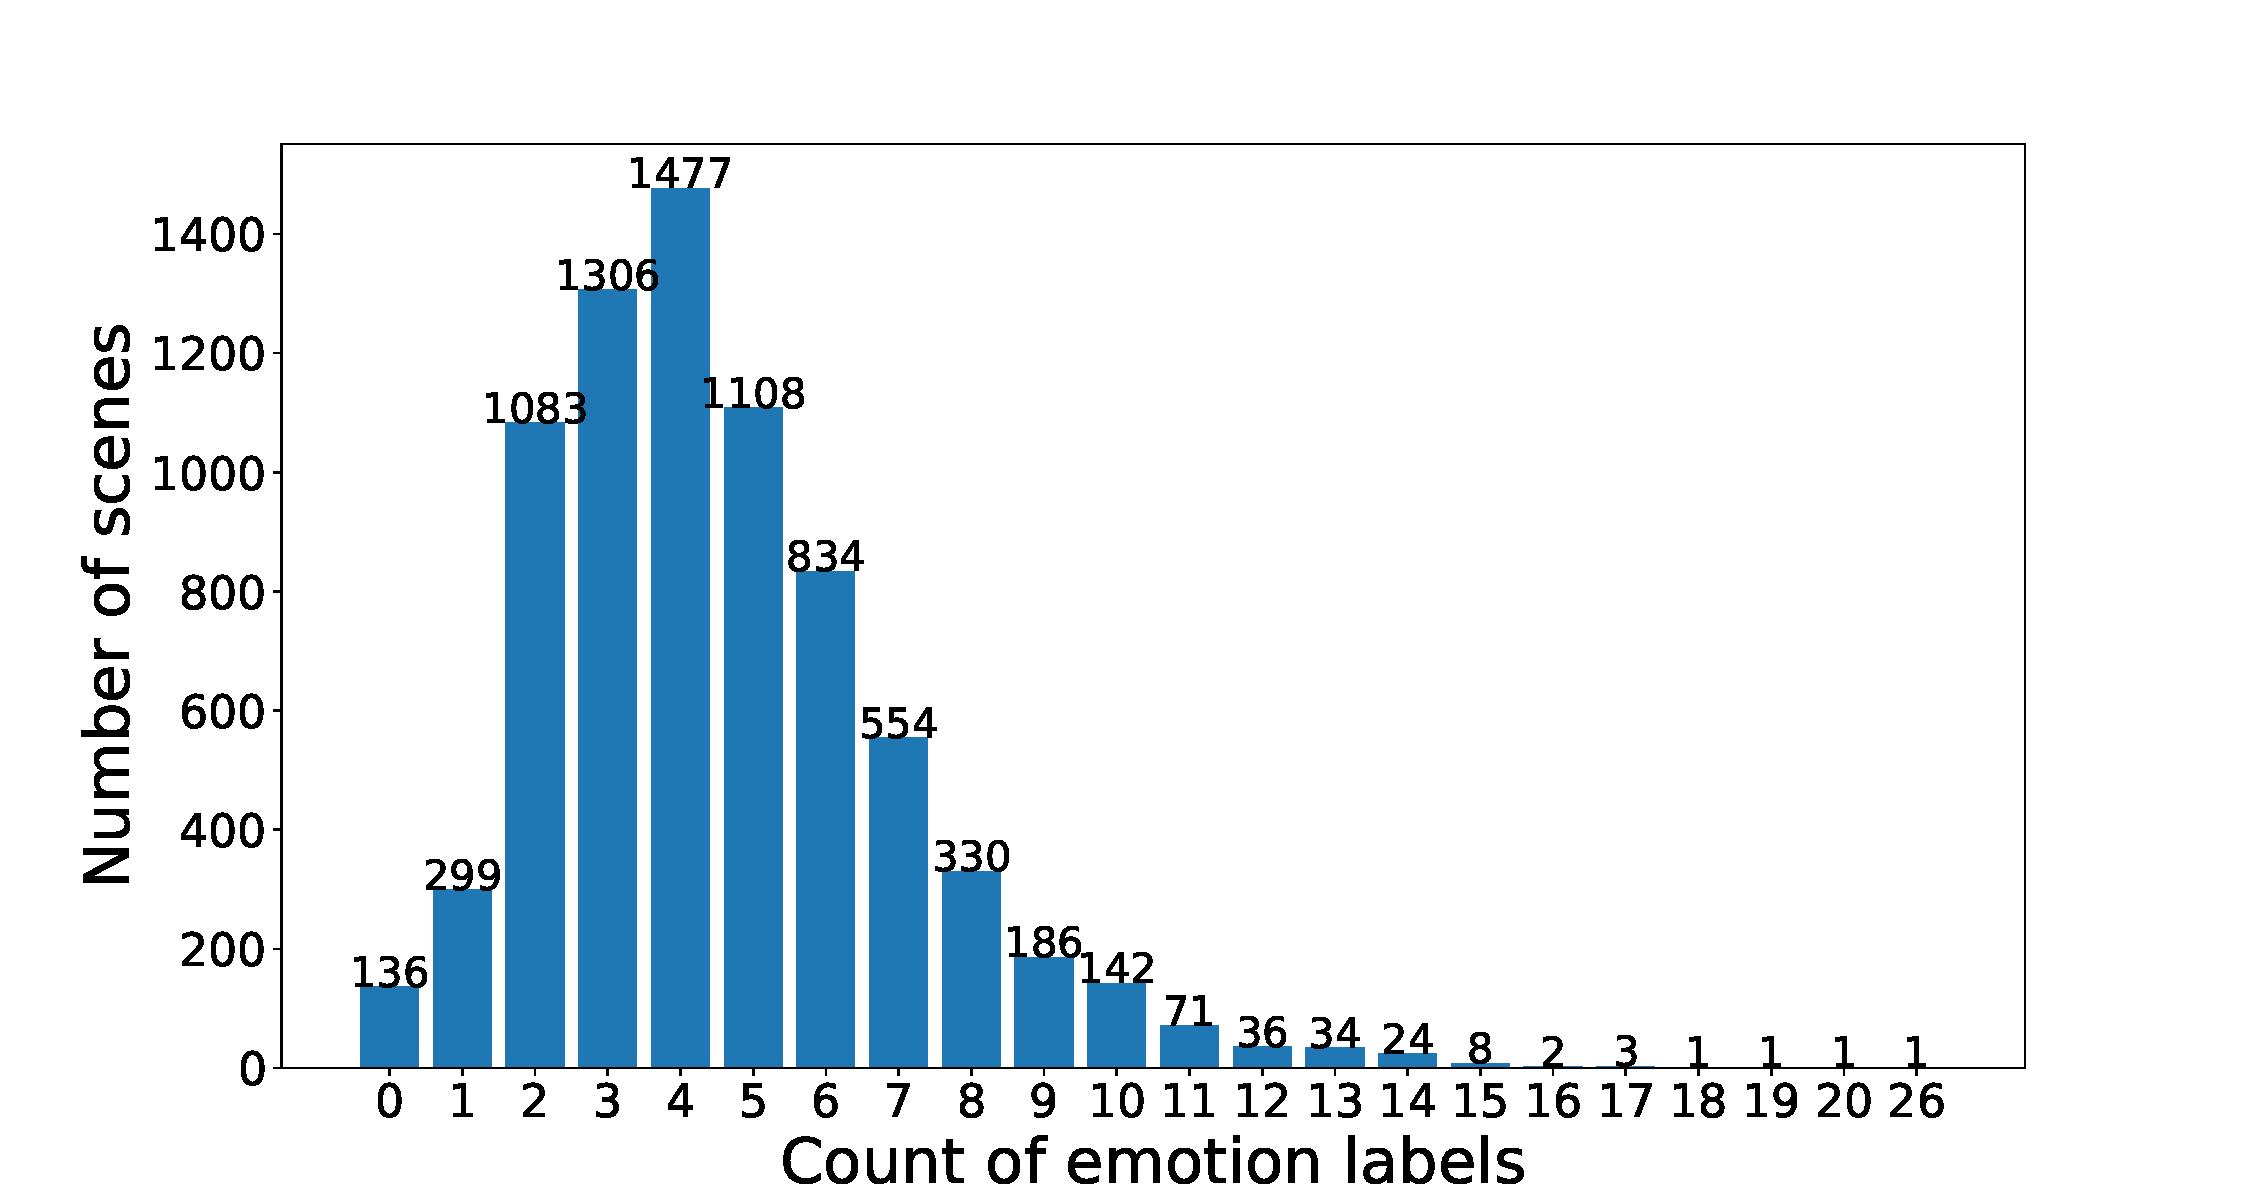
\includegraphics[width=0.7\linewidth]{Figures/emo_counts_in_ClipGraphs.pdf}
\vspace{-2mm}
\caption{Bar chart showing the number of movie scenes associated with a specific count of annotated emotions.}
\vspace{-5mm}
\label{fig:emotion_count_distribution}
\end{figure}

We use the MovieGraphs dataset~\cite{moviegraphs} that features 51 movies and 7637 movie scenes with detailed graph annotations.
We focus on the list of characters and their emotions and mental states, which naturally affords a multi-label setup.
Other annotations such as the situation label, or character interactions and relationships~\cite{lirec} are ignored as they cannot be assumed to be available for a new movie.

\paragraph{Label sets.}
Like other annotations in the MovieGraphs dataset, emotions are also obtained as free-text leading to a huge variability and a long-tail of labels (over 500).
We focus our experiments on three types of label sets:
(i)~\emph{Top-10} considers the most frequently occurring 10 emotions;
(ii)~\emph{Top-25} considers frequently occurring 25 labels; and
(iii)~\emph{Emotic}, a mapping from 181 MovieGraphs emotions to 26 Emotic labels provided by~\cite{affect2mm}. In Fig.~\ref{fig:emotionFrequency} we show the number of movie scenes that contain top-10 and 25 emotions.

\paragraph{Statistics.}
We first present row max-normalized co-occurrence matrices for the scene and characters (Fig.~\ref{fig:cooccurrence_maps}).
It is interesting to note how a movie scene has high co-occurrence scores for emotions such as \emph{worried} and \emph{calm} (perhaps owing to multiple characters), while \emph{worried} is most associated with \emph{confused} for a single character.
Another high scoring example for a single character is \emph{curious} and \emph{surprise},
while a movie scene has \emph{curious} with \emph{calm} and \emph{surprise} with \emph{happy}.
In Fig.~\ref{fig:emotion_count_distribution}, we show the number of movie scenes that contain a specified number of emotions.
Most scenes have 4 emotions.

\paragraph{Evaluation metric.}
We use the original splits from MovieGraphs.
As we have $K$ binary classification problems, we adopt mean Average Precision (mAP) to measure model performance (similar to Atomic Visual Actions~\cite{ava}).
Note that AP also depends on the label frequency.
